\documentclass[a4paper]{report}
% Shared preamble for the English probability and statistics documents.
% Based on the original course preamble. Compile with pdfLaTeX.
\usepackage[top=1.5cm,bottom=2cm,left=2cm,right=2cm]{geometry}
\usepackage[T1]{fontenc}
\usepackage{lmodern}
\usepackage[utf8]{inputenc}
\usepackage[english]{babel}

\usepackage{amsmath}
\usepackage{amssymb}
\usepackage{amsthm}
\usepackage{mathrsfs}
\usepackage{mathtools}
\usepackage{etoolbox}
\usepackage{tikz}
\usetikzlibrary{shapes.multipart,arrows.meta}
\usepackage{xcolor}
\usepackage{enumerate}
\usepackage[shortlabels]{enumitem}
\usepackage{hyperref}
\usepackage{version}
\usepackage{bbold}
\usepackage{fontawesome5}
\usepackage{fancyhdr}
\lfoot{}
\usepackage{natbib}
\usepackage{graphicx}
\usepackage{pdfpages}
\usepackage{authblk}
    
\usepackage{blindtext}
\usepackage{multicol}
\usepackage{collcell}
\usepackage{wrapfig}
\usepackage{blkarray}
\usepackage{cancel}
\usepackage{appendix}
\usepackage{float}
\makeatletter
\input{tex/assets/slashbox.sty}
\makeatother
\hypersetup{unicode,colorlinks,citecolor=red,filecolor=black,
  linkcolor=red,urlcolor=cyan}
\setlength{\columnsep}{1cm}
\pagenumbering{gobble}

\def\numtext#1{%
  \ifcase#1\or one\or two\or three\or four\or five\or six\or seven\or eight\or nine\or ten\or
  eleven\or twelve\or thirteen\or fourteen\or fifteen\or sixteen\or seventeen\or eighteen\or nineteen\or twenty\or Lots\fi}

\newcommand{\Byte}[1]{%
  \def\nodecontents{}%
  \foreach[count=\l] \k in {#1} {\xappto{\nodecontents}{\noexpand\nodepart{\numtext{\l}}\k}}%
  \node[rectangle split,rectangle split parts=8,rectangle split horizontal,draw] at (2,2){\nodecontents};}

\newcommand{\D}{{\mathrm{d}}}
\newcommand{\cE}{{\mathcal{E}}}
\newcommand{\cG}{{\mathcal{G}}}
\newcommand{\cX}{{\mathcal{X}}}
\newcommand{\cY}{{\mathcal{Y}}}
\newcommand{\cB}{{\mathcal{B}}}
\newcommand{\cF}{{\mathcal{F}}}
\newcommand{\cO}{{\mathcal{O}}}
\newcommand{\cS}{{\mathcal{S}}}
\newcommand{\cT}{{\mathcal{T}}}
\newcommand{\given}{\, \big| \,}
\newcommand{\cL}{{\mathscr{L}}}
\newcommand{\cD}{{\mathcal{D}}}
\newcommand{\cA}{{\mathscr{A}}}
\newcommand{\cP}{{\mathscr{P}}}
\newcommand{\cR}{{\mathscr{R}}}
\newcommand{\A}{{\mathcal A}}
\newcommand{\one}{\mathbb{1}}
\newcommand{\mathbbm}[1]{\mathbb{#1}}

\providecommand{\C}{}
\renewcommand{\C}{\mathbb C}
\newcommand{\R}{\mathbb R}
\newcommand{\Q}{\mathbb Q}
\newcommand{\N}{\mathbb N}
\newcommand{\T}{\mathbb T}
\newcommand{\F}{\mathbb F}
\renewcommand{\P}{\mathbb P}
\newcommand{\Z}{\mathbb Z}
\newcommand{\E}{\mathbb {E}}
\newcommand{\Pbb}[1]{\P\left( #1\right)}
\newcommand{\Ebb}[1]{\E\left[ #1\right]}

\newcommand{\lb}{\left (}
\newcommand{\rb}{\right )}
\newcommand{\lbb}{\left [}
\newcommand{\rbb}{\right ]}
\newcommand{\labs}{\left |}
\newcommand{\rabs}{\right |}
\newcommand{\lbrb}[1]{\lb #1 \rb}
\newcommand{\lbbrbb}[1]{\lbb#1\rbb}
\newcommand{\labsrabs}[1]{\labs#1\rabs}
\newcommand{\lbbrb}[1]{\lbb#1\rb}
\newcommand{\lbrbb}[1]{\lb#1\rbb}
\newcommand{\langlerangle}[1]{\langle#1\rangle}
\newcommand{\lbcurly}{\{}
\newcommand{\rbcurly}{\}}
\newcommand{\curly}[1]{\lbcurly#1\rbcurly}
\newcommand{\abs}{\labsrabs}
\newcommand{\ind}[1]{1_{#1}}
\newcommand{\indep}{\perp \!\!\! \perp}
\renewcommand{\d}{\, \mathrm{d}}

\newtheorem{theorem}{Theorem}
\newtheorem{problemCnt}{Lemma}
\theoremstyle{definition}
\newtheorem{problem}[problemCnt]{Problem}
\newtheorem{problembook}[problemCnt]{\faBook \,  Problem}
\newtheorem{problempencil}[problemCnt]{\faPencil* \,  Problem}
\newtheorem{problemstar}[problemCnt]{\faStar\,  Problem}
\newtheorem{problemstarpencil}[problemCnt]{\faStar \, \faPencil* \,   Problem}
\newtheorem{probleminteresting}[problemCnt]{\faSmile[regular] \,   Problem}
\newtheorem{solution}{Solution}

\newcommand{\fwcell}[1]{\makebox[\arraystretch\normalbaselineskip]{$#1$}}
\newenvironment{enumeratei}{\begin{enumerate}[(i)]}{\end{enumerate}}
\newenvironment{enumeratea}{\begin{enumerate}[(a)]}{\end{enumerate}}
\newenvironment{enumeraten}{\begin{enumerate}[\upshape 1.]}{\end{enumerate}}

% Compatibility helpers needed by a few files in the combined archive.
\AtBeginDocument{\noindent{\footnotesize English translation prepared with ChatGPT (OpenAI, GPT-6), 26 October 2026, for translation of the Bulgarian text into English and LaTeX formatting.
The Bulgarian originals remain the reference; translation may contain errors.}\par\smallskip}
\newcommand{\MissingGraphic}[1]{%
  \begin{center}\fbox{\parbox{0.82\linewidth}{\centering Missing source image: \texttt{#1}}}\end{center}}



\begin{document}
\noindent Applied Mathematics / Mathematics, 14 June 2026 \hfill Written examination
\hrulefill
\begin{it}The exact grading formula will depend on the results. As an approximation, use 2 + the number of points. Every answer must be justified and supported by clear, detailed calculations. Electronic devices (except standard calculators) and additional materials are prohibited. Time allowed: 4 hours. Good luck!\end{it}
\begin{problem} (1.5 points)~
\begin{enumerate}
\item (0.5 points) Let $Y\sim\mathrm{Geo}(q)$\footnote{Use the convention ``number of failures before the first success''.} and let $X\mid Y=n\sim\mathrm{NB}(n+1,q)$. Find the distribution, expectation and probability generating function of $X$.\footnote{Recall $\sum_{j=0}^\infty\binom{m+j-1}{m-1}x^j=(1-x)^{-m}$ for $|x|<1$ and $m\in\mathbb N$.}
\item (0.5 points) Find the expected number of tosses of a coin with probability $p$ of heads until two consecutive tails first occur.
\emph{Hint:} You may use the preceding parts.
\[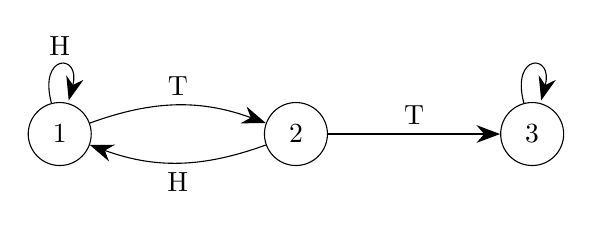
\begin{tikzpicture}[>={Stealth[length=3mm]},vertex/.style={circle,draw,minimum size=8mm}]
\node[vertex](1)at(0,0){1};\node[vertex](2)at(3,0){2};\node[vertex](3)at(6,0){3};
\draw[->](1)edge[loop above]node[above]{H}();\draw[->](3)edge[loop above]();
\draw[->,bend left=20](1)to node[midway,above]{T}(2);
\draw[->,bend left=20](2)to node[midway,below]{H}(1);
\draw[->](2)--node[midway,above]{T}(3);
\end{tikzpicture}\]
\item (0.5 points) Find the expected number of occurrences of two consecutive tails in $n\geq2$ tosses.
\end{enumerate}
\end{problem}
\begin{problem} (1 point)
Independently choose two points on the axes of a Cartesian coordinate system: $A$ has a standard normal distribution on the horizontal axis and $B$ on the vertical axis.\footnote{Equivalently, use the points $(A,0)$ and $(0,B)$, where $A,B\overset{iid}{\sim}N(0,1)$.}
\begin{enumerate}
\item (0.25 points) Find the distribution and expectation of $|A|$.
\item (0.75 points) Find the probability that $(A,B)$ lies in the disc of radius 4 centred at $(0,0)$. What is the probability that $\angle OAB\leq\pi/4$?
\end{enumerate}
\end{problem}
\begin{problem} (1.25 points)
\begin{enumerate}
\item (0.75 points) Let $X_1,\ldots,X_n$ be iid with density $f(x;\theta)=2x/\theta^2$ for $0<x<\theta$, and 0 otherwise, where $\theta>0$. Find the maximum likelihood estimator of $\theta$ and check whether it is unbiased and consistent.
\item (0.5 points) Let $X_1,\ldots,X_n\overset{iid}{\sim}\mathrm{Gamma}(\alpha,\beta)$, where $\alpha,\beta>0$, with density $f(x)=\beta^\alpha x^{\alpha-1}e^{-\beta x}/\Gamma(\alpha)$ for $x>0$, and 0 otherwise. Find method of moments estimators of $\alpha,\beta$.
\end{enumerate}
\end{problem}
\begin{problem} (1.25 points)~
\begin{enumerate}
\item (0.25 points) A box contains 5 red, 4 blue and 3 green balls. Select 4 without replacement. Find the probability of selecting at least one of each colour.
\item (0.5 points) Let $(X,Y)$ have joint density
\[f_{X,Y}(x,y)=\begin{cases}cxy,&0<x<1,\ x^2<y<\sqrt x,\\0,&\text{otherwise.}\end{cases}\]
Find $c$, $\E[X]$, $\E[X\mid Y=1/4]$ and $\P(X+Y<1)$.
\item (0.25 points) Let $X_n\sim\mathrm{Exp}(n)$ for $n\in\mathbb N$. Show that $X_n$ converges in probability. Find the limiting distribution of $nX_n$.
\item (0.25 points) Let $\Theta\sim\mathrm{Exp}(\lambda)$ and $X\mid\Theta=\theta\sim\mathrm{Po}(\theta)$, with $\lambda>0$. Find the conditional density of $\Theta\mid X=x$.
\end{enumerate}
\end{problem}
\end{document}
